
\section{Installing on Linux}

Note:  This is written for version 5.6.  With 5.9 things should change
significantly, both for Windows and Linux, so a rewrite will be performed
at that time.

\subsection{The Easy Way}

If you are using Debian Linux, there are packages for Maxima in the
Debian archives. Redhat users can find packages at rpmfind.net and
mirrors. To the best of my knowledge these packages are all compiled
against GNU Common Lisp (GCL). GCL does not access the readline library,
which makes using Maxima on the terminal somewhat cumbersome. There
are various interfaces which address this issue, but in the case of
these packages the left arrow key will not take you back to the middle
of an expression and let you edit just what you want - you will have
to delete everything back to the point where you made your error.
See the interfaces section for more about this, or if you really want
to use maxima in the terminal I'd recommend compiling against CLISP. 


\subsection{The Hard Way}

Compiling Maxima on Linux should go reasonably smoothly, although
some distributions seem to have problems with the makefiles. Redhat
7.1 is known to be a bit flaky in this regard.


\subsubsection{Compiling with GCL\index{Compiling!GCL} }

GCL is the version of Lisp Maxima has been maintained on for many
years by William Schelter, and thus the default system on which to
build Maxima. Maxima will typically be made to work with GCL, and
then be fixed to work with other Lisps. If in doubt, start here, but
again be warned that readline support is not present in GCL.

The first step in this process is to compile GCL. The files from the
compiling of GCL are needed when building Maxima against it, so first
download and decompress the most current version of GCL. Compiling
it should be simple:

\vspace{3ex}


cd \$HOME/gcl

./configure

make\vspace{3ex}


Once that is complete, download and decompress Maxima. Now the process
gets a little more complicated - you will have to hand edit the file
\texttt{configure}. What follows is the first part of the file, with
the parts you must edit in bold:

\vspace{3ex}%

\#!/bin/sh

\# edit next few lines 

\# GCLDIR should be where gcl was built, and the o/{*}.o lsp/{*}.o
etc must be

\# there to link with maxima

GCLDIR=\textbf{/home/cliff/gcl-2.3.8}

\# the directory where this file is, and where you will build maxima

\# could use

MAXDIR=\textbf{/home/cliff/maxima-5.5}

MAXDIR=`pwd`

\# where to put some maxima .el files

EMACS\_SITE\_LISP=\textbf{/usr/lib/emacs/site-lisp}

\# determines where to install

\# PREFIX\_DIR=/usr/local puts things in /usr/local/lib/maxima-x.y

\# and /usr/local/bin

PREFIX\_DIR=\textbf{/usr/local}

INFO\_DIR=\$\{PREFIX\_DIR\}/info

MAN\_DIR=\$\{PREFIX\_DIR\}/man/man1

\#\#\#\#\# end editing \#\#\#\#\#\#\#\#\#

\vspace{3ex}%

Once this is correctly done, run the configure script: \texttt{./configure.}
If this succeeds without any problems, run \texttt{make}. This could
be a long process, depending on your machine. Once it is done, and
if no errors result, run \texttt{make test}. If any errors appear
in either stage, consult the trouble shooting section. Otherwise,
you are ready to su into root and run \texttt{make install}. Once
this process is completed, you should be able to run \texttt{maxima}
and \texttt{xmaxima}. Emacs mode may take a little more work, and
the other interfaces are separate programs - see the Interfaces chapter
for details.


\subsubsection{Compiling with CLISP\index{Compiling!CLISP}}

Clisp has, among other features, the ability to use the readline library.
This means that many of the limitations created in the terminal by
GCL are not relevant here, and for the beginner especially this is
a good place to start. Unfortunately, compiling on a flavor of Lisp
other than GCL is not quite as smooth - here are the steps. 

Change into the directory \$HOME/maxima/src (or \$HOME/maxima-5.6/src
- whatever your setup dictates.)

For newer versions of clisp, you need to change a couple lines in
the file compile-clisp.lisp:

\vspace{3ex}

< (lisp:gc) \( \rightarrow  \) (ext:gc)

< (lisp:saveinitmem \char`\"{}maxima-clisp.mem\char`\"{} \( \rightarrow  \)
(ext:saveinitmem \char`\"{}maxima-clisp.mem\char`\"{}

\vspace{3ex}

Then run the following commands:

\vspace{3ex}

make clisp-compile CLISP=clisp

make maxima-clisp.mem CLISP=clisp

make test-clisp CLISP=clisp

\vspace{3ex}

Once that is complete, you can either leave maxima where you built
it, or move the directory to a more suitable place. Once that is done,
in order to set up a convenient way to run Maxima, you can create
some shell scripts in /usr/local/bin (make sure to do chmod +x on
both files):

\vspace{3ex}

===================maxima==============

\#!/bin/bash

export~MAXIMA\_DIRECTORY=/PATH\_TO\_NEW\_DIRECTORY/maxima

exec~clisp~-M~\$\{MAXIMA\_DIRECTORY\}/src/maxima-clisp.mem 

=======================================

\vspace{3ex}

===============xmaxima==================

\#!/bin/bash

export~MAXIMA\_DIRECTORY=/PATH\_TO\_NEW\_DIRECTORY/maxima

exec~\$\{MAXIMA\_DIRECTORY\}/bin/xmaxima~-lisp~clisp

=======================================

\vspace{3ex}


\subsubsection{Compiling with CMULISP\index{Compiling!CMULISP}}


\subsubsection{Other Lisps}


\section{Installing on Windows}


\subsection{The Easy Way - Installing the Windows Binary }

This is the recommended way to use Maxima on Windows. The current
binary release is technically a beta, but should serve most needs
quite well. Here is how a basic install works:

\begin{enumerate}
\item Download the binary from http://www.ma.utexas.edu/maxima.html
It should be named maxima55l-setup.exe
\item Once you have downloaded that file, launch the installer. You
should see this screen:
\end{enumerate}
\vspace{0.3cm}
{\centering 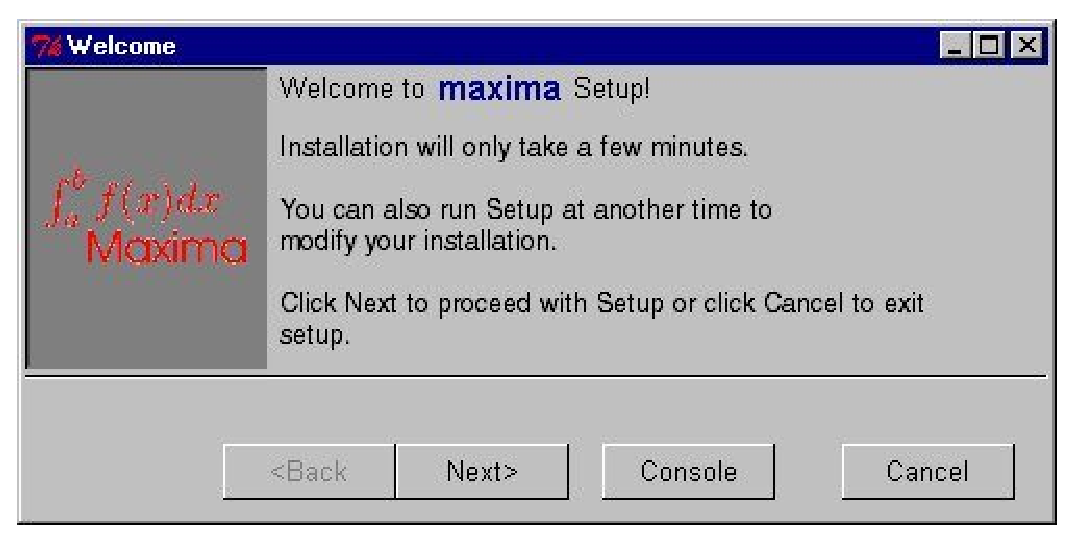
\includegraphics{images/maximawindowsinstall1}}
\vspace{0.3cm}
\begin{enumerate}
\item [3.]Simply follow the menus from that point - the install dialog
should be very clear. Do read the README and License when they are
presented - the information there is good to know.
\item [4.]Simply launch the program from it's icon - everything should work
out of box. It is known to run on the following versions of Windows:

\vspace{3ex}

Windows 98

\end{enumerate}

\subsection{The Hard Way}

Compiling on Windows (I have no idea how to do this.)
